\documentclass{ctexart}
\usepackage{amsmath, amsfonts, amssymb} % 数学公式、符号
\usepackage[colorlinks,linkcolor=red,anchorcolor=blue,citecolor=green]{hyperref}
\usepackage[left=2.50cm, right=2.50cm, top=2.50cm, bottom=2.50cm]{geometry} %页边距
\usepackage{graphicx}   % 图片
\usepackage{multicol}
\usepackage{bm}
\usepackage{listings}
\usepackage{xcolor}
\usepackage{tikz}
\usetikzlibrary{arrows,shapes,chains}
\usepackage{multirow}
\usepackage{fancyhdr} %设置页眉、页脚
\pagestyle{fancy}
\lhead{}
\chead{}
\lfoot{}
\cfoot{}
\rfoot{}

% 用来设置代码的样式
\lstset{
	basicstyle          =   \sffamily,          % 基本代码风格
	keywordstyle        =   \bfseries,          % 关键字风格
	commentstyle        =   \rmfamily\itshape,  % 注释的风格,斜体
	stringstyle         =   \ttfamily,  % 字符串风格
	flexiblecolumns,                % 别问为什么,加上这个
	numbers             =   left,   % 行号的位置在左边
	showspaces          =   false,  % 是否显示空格,显示了有点乱,所以不现实了
	numberstyle         =   \zihao{-5}\ttfamily,    % 行号的样式,小五号,tt等宽字体
	showstringspaces    =   false,
	captionpos          =   t,      % 这段代码的名字所呈现的位置,t指的是top上面
	frame               =   lrtb,   % 显示边框
}

\lstdefinestyle{Python}{
	language        =   Python, % 语言选Python
	basicstyle      =   \zihao{-5}\ttfamily,
	numberstyle     =   \zihao{-5}\ttfamily,
	keywordstyle    =   \color{blue},
	keywordstyle    =   [2] \color{teal},
	stringstyle     =   \color{magenta},
	commentstyle    =   \color{red}\ttfamily,
	breaklines      =   true,   % 自动换行,建议不要写太长的行
	columns         =   fixed,  % 如果不加这一句,字间距就不固定,很丑,必须加
	basewidth       =   0.5em,
}

\title{\textbf{机器学习实验报告\\{\Large{线性模型}}}} % 标题与子标题
\author{\sffamily{朱天泽}} % 作者
\date{(日期:\today)} % 日期

\begin{document}
	\maketitle\thispagestyle{fancy}
	% 摘要开始
	\noindent{\bf{摘要}}
		在《机器学习》第三章中,我学习了诸多线性模型。在此次实验中,我尝试用Python语言实现了对率回归、线性判别分析(LDA)等线性模型,并给出了其在西瓜数据集 $3.0\alpha$ 上的结果。此外,我尝试使用了机器学习库scikit-learn,同自己实现的算法进行了比较。
		
	\noindent{\bf{关键词}} 对率回归;LDA;分类;scikit-learn;
	
	% 正文开始
	\section{习题3.3}
	\subsection{编程题目理解}
	题目要求编程实现对数几率回归,并给出西瓜数据集 $3.0\alpha$ 上的结果。
	
	在西瓜数据集 $3.0\alpha$ 中,西瓜包含“密度”和“含糖率”两个参数,因此可将西瓜看做横坐标为“密度”纵坐标为“含糖率”的坐标系中的点,记为 $\bm{x}=(x_1,x_2)$。我们使用该数据,找到合适的 $(\bm{w},b)$,利用对数几率函数 $\frac{1}{1+e^{-z}}$ 对西瓜进行二分类(好瓜、坏瓜)。
	\subsection{对数几率回归原理阐述}
	已知单调可微函数 $g(\cdot)$,令 $y=g^{-1}(\bm{w}^\mathrm{T}\bm{x}+b)$,这样得到的模型称为“广义线性模型”。
	
	\begin{figure}[htb]
		\centering
		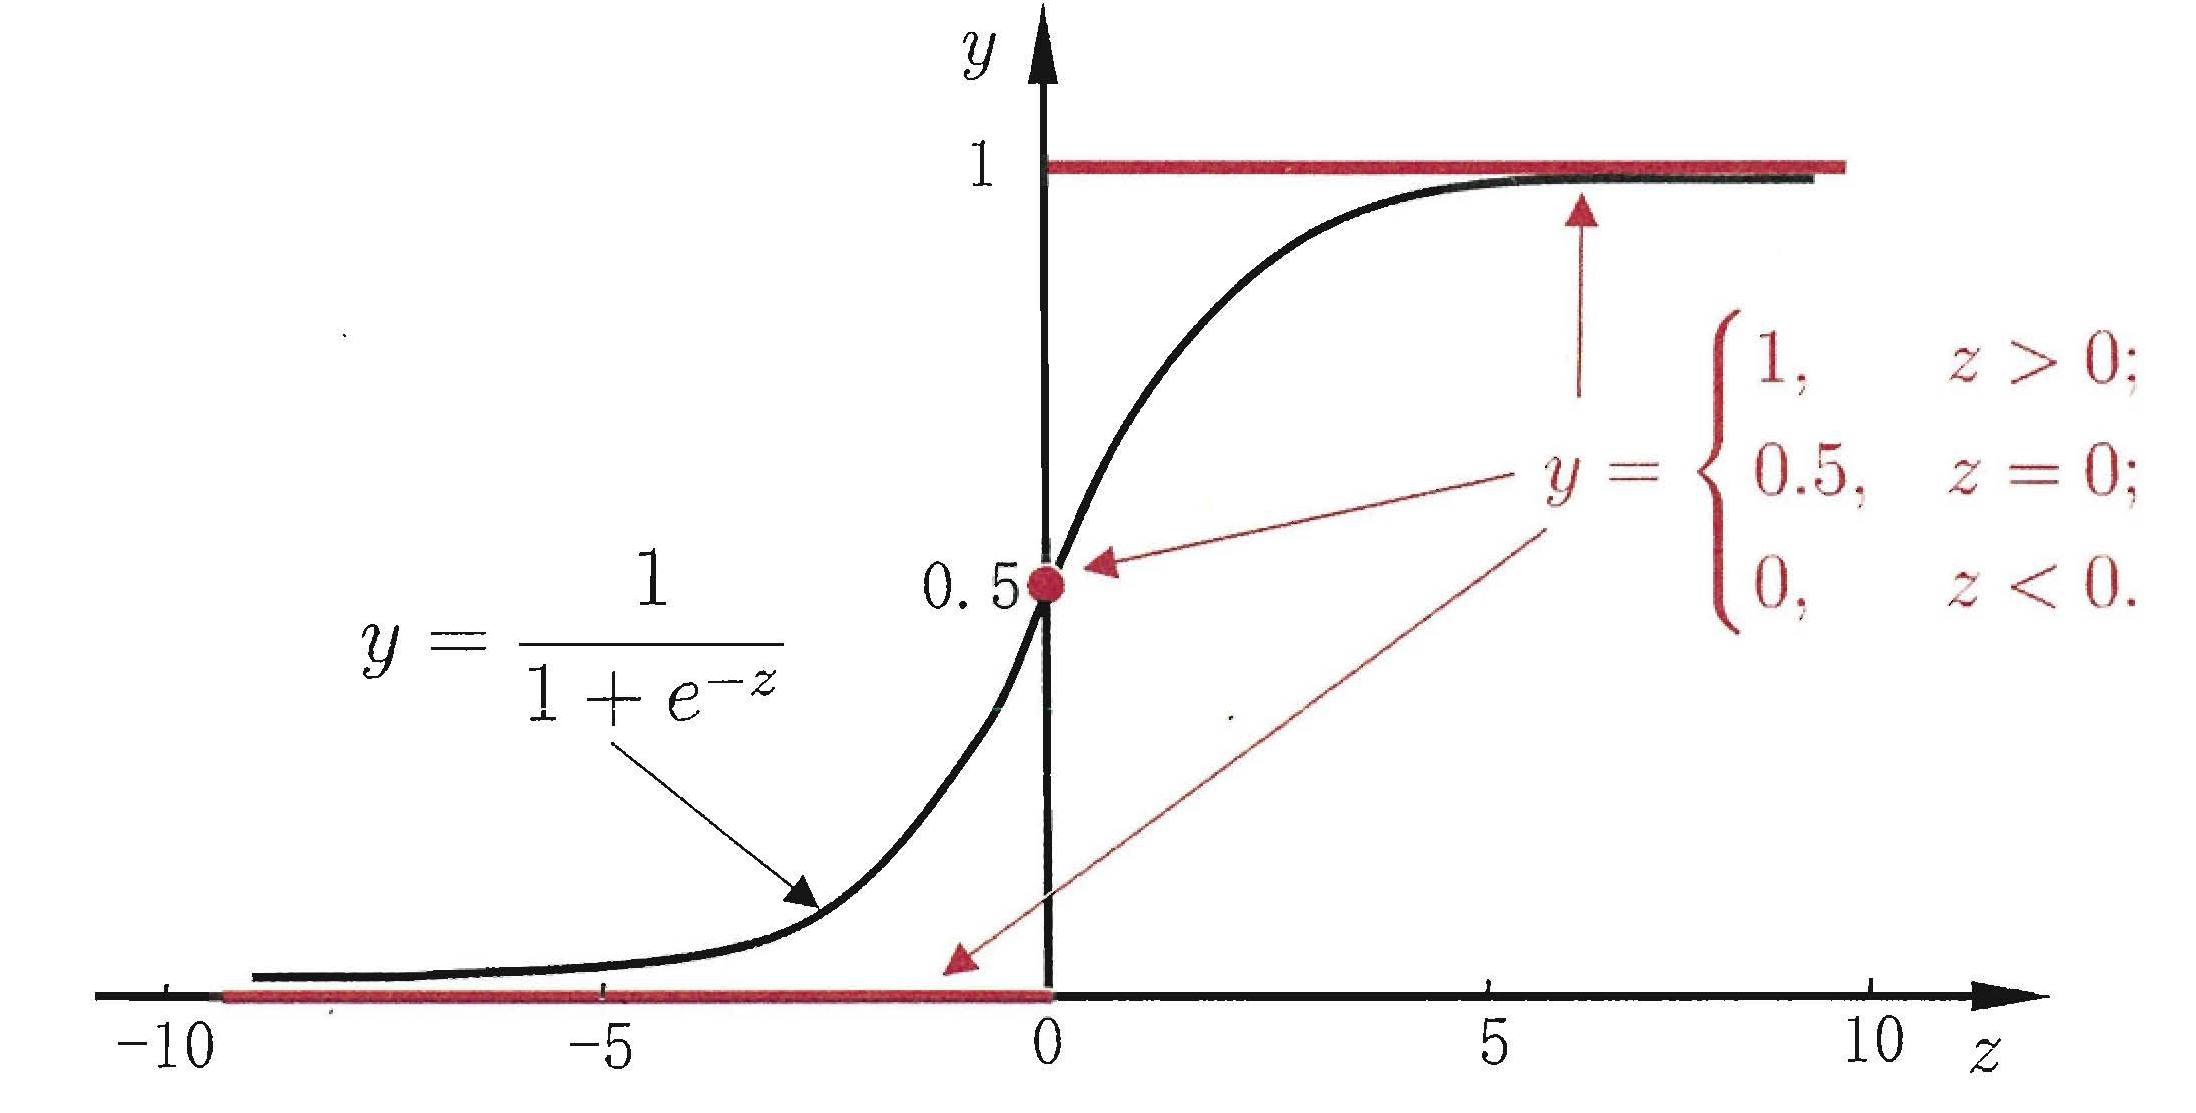
\includegraphics[scale=1,height=6cm]{../image/Logistic.png}
		\caption{单位跃阶函数与对数几率函数}
		\label{Image_Logistic}
	\end{figure}
	
	考虑二分类任务,其输出标记 $y\in\{0,1\}$,而线性回归模型阐述的预测值 $z=\bm{w}^\mathrm{T}\bm{x}+b$;将 $z$ 映射为 $0/1$ 值,最理想的是“单位越阶函数” $y=\begin{cases}0&z<0\\0.5&z=1\\1&z>1\end{cases}$。可以看到单位跃阶函数并不连续,不能作为广义线性模型中的 $g^{-1}(\cdot)$,因此我们用对数几率函数 $y=\frac{1}{1+e^{-z}}$ 来近似单位跃阶函数,如图\ref{Image_Logistic}。
	

	从图\ref{Image_Logistic}可以看出,对数几率函数将预测值$z$转化为一个接近0或1的$y$值,并且其输出值在$z=0$附近变化剧烈。将 $z$ 代入对数几率函数,得到
	
	\begin{equation}
		y=\frac{1}{1+e^{-(\bm{w}^\mathrm{T}\bm{x}+b)}}
		\label{Initial_Logistic}
	\end{equation}

	式\eqref{Initial_Logistic}有很好的性质,即
	
	\begin{equation}
		\left\{\begin{matrix}
		y=\frac{1}{1+e^{-(\bm{w}^\mathrm{T}\bm{x}+b)}}	\\
		1-y=\frac{e^{-(\bm{w}^\mathrm{T}\bm{x}+b)}}{1+e^{-(\bm{w}^\mathrm{T}\bm{x}+b)}}
		\end{matrix}\right.
		\label{Good_Logistic}
	\end{equation}
	
	式\eqref{Good_Logistic}可进一步等价为
	
	\begin{equation}
		\ln\frac{y}{1-y}=\bm{w}^\mathrm{T}\bm{x}+b
		\label{Log_Ratio}
	\end{equation}

	若将$y$视为样本$\bm{x}$作为正例的可能性,则$1-y$是其为反例的可能性,两者的比值$\frac{y}{1-y}$称为“几率”,那么式\eqref{Log_Ratio}就称为“对数几率”。
	
	我们将式\eqref{Initial_Logistic}中的$y$视为类后验概率估计$p(y=1|\bm{x})$,将式\eqref{Initial_Logistic}分子分母同乘$e^{\bm{w}^\mathrm{T}\bm{x}+b}$,显然有
	
	\begin{equation}
		\begin{aligned}
			p(y=1|\bm{x})=\frac{e^{\bm{w}^\mathrm{T}\bm{x}+b}}{1+e^{\bm{w}^\mathrm{T}\bm{x}+b}}\\
			p(y=0|\bm{x})=\frac{1}{1+e^{\bm{w}^\mathrm{T}\bm{x}+b}}
		\end{aligned}
	\end{equation}

	于是,我们可以通过“极大似然法”来估计$\bm{w}$和$b$。给定数据集$\{\bm{x}_i,y_i\}_{i=1}^m$,对数几率回归模型最大化“对数似然”
	
	\begin{equation}
		\ell(\bm{w},b)=\sum_{i=1}^m\ln p(y_i|\bm{x}_i;\bm{w},b)
		\label{Likelyhood}
	\end{equation}

	即令每个样本属于真实标记的概率越大越好。为方便讨论,令 $\bm{\beta}=(\bm{w};b)$,$\hat{\bm{x}}=(\bm{x};1)$;再令 $p_{y^\ast}(\hat{\bm{x}};\bm{\beta})=p(y=y^\ast|\hat{\bm{x}};\bm{\beta})$,则式\eqref{Likelyhood}中的似然项可改写为
	
	\begin{equation}
		p(y_i|\bm{x}_i;\bm{w},b)=(p_1(\hat{\bm{x}}_i;\bm{\beta})^{y_i})(p_0(\hat{\bm{x}}_i;\bm{\beta}))^{1-y_i}
		\label{Cool_Likelyhood}
	\end{equation}

	将式\eqref{Cool_Likelyhood}代回式\eqref{Likelyhood},得
	
	\begin{equation}
		\begin{aligned}
			\ell(\bm{\beta})&=\sum_{i=1}^m\ln[(p_1(\hat{\bm{x}}_i;\bm{\beta})^{y_i})(p_0(\hat{\bm{x}}_i;\bm{\beta}))^{1-y_i}]\\
			&=\sum_{i=1}^m[y_i\ln(p_1(\hat{\bm{x}}_i;\bm{\beta}))+(1-y_i)\ln(p_0(\hat{\bm{x}}_i;\bm{\beta}))]\\
			&=\sum_{i=1}^m\{y_i[\ln(p_1(\hat{\bm{x}}_i;\bm{\beta}))-\ln(p_0(\hat{\bm{x}}_i;\bm{\beta}))]+\ln(p_0(\hat{\bm{x}}_i;\bm{\beta}))\} \\
			&=\sum_{i=1}^m\left[y_i\ln\left(\frac{p_1(\hat{\bm{x}}_i;\bm{\beta})}{p_0(\hat{\bm{x}}_i;\bm{\beta})}\right)+\ln(p_0(\hat{\bm{x}}_i;\bm{\beta}))\right]\\
			&=\sum_{i=1}^m\left[y_i\ln\left(e^{\bm{\beta}^\mathrm{T}\hat{\bm{x}}_i}\right)+\ln\left(\frac{1}{1+e^{\bm{\beta}^\mathrm{T}\hat{\bm{x}}_i}}\right)\right] \\
			&=\sum_{i=1}^m\left[y_i\bm{\beta}^\mathrm{T}\hat{\bm{x}}_i-\ln\left(1+e^{\bm{\beta}^\mathrm{T}\hat{\bm{x}}_i}\right)\right]
		\end{aligned}
		\label{Initial_LB}
	\end{equation}
	
	最大化式\eqref{Initial_LB}等价于最小化
	
	\begin{equation}
		\ell(\bm{\beta})=\sum_{i=1}^m\left[-y_i\bm{\beta}^\mathrm{T}\hat{\bm{x}}_i+\ln\left(1+e^{\bm{\beta}^\mathrm{T}\hat{\bm{x}}_i}\right)\right]
		\label{Need_Cal}
	\end{equation}
	
	式\eqref{Need_Cal}是关于$\bm{\beta}$的高阶可导连续凸函数。因此当$\frac{\partial\ell(\bm{\beta})}{\partial\bm{\beta}}=0$时,解得 $\bm{\beta}^\ast=\arg\min\limits_{\bm{\beta}}\ell(\bm{\beta})$。
	
	我们可以使用牛顿迭代法求解$\frac{\partial\ell(\bm{\beta})}{\partial\bm{\beta}}=0$。迭代式为
	
	\begin{equation}
		\bm{\beta}'=\bm{\beta}-\left(\frac{\partial^2\ell(\bm{\beta})}{\partial\bm{\beta}\partial\bm{\beta}^\mathrm{T}}\right)^{-1}\frac{\partial\ell(\bm{\beta})}{\partial\bm{\beta}}
		\label{Iter}
	\end{equation}

	\begin{equation}
		\begin{aligned}
			\frac{\partial\ell(\bm{\beta})}{\partial\bm{\beta}}&=\sum_{i=1}^m\left[-y_i\frac{\partial\left(\bm{\beta}^{\mathrm{T}}\hat{\bm{x}}_i\right)}{\partial\bm{\beta}}+\frac{\partial\ln\left(1+e^{\bm{\beta}^\mathrm{T}\hat{\bm{x}}_i}\right)}{\partial\bm{\beta}}\right]\\
			&=\sum_{i=1}^m\left[-y_i\hat{\bm{x}}_i+\frac{1}{1+e^{\bm{\beta}^\mathrm{T}\hat{\bm{x}}_i}}\frac{\partial(1+e^{\bm{\beta}^\mathrm{T}\hat{\bm{x}}_i})}{\partial\bm{\beta}}\right]\\
			&=\sum_{i=1}^m\left(-y_i\hat{\bm{x}}_i+\frac{e^{\bm{\beta}^\mathrm{T}\hat{\bm{x}}_i}\hat{\bm{x}}_i}{1+e^{\bm{\beta}^\mathrm{T}\hat{\bm{x}}_i}}\right)\\
			&=-\sum_{i=1}^m\hat{\bm{x}}_i\left(y_i-\frac{e^{\bm{\beta}^\mathrm{T}\hat{\bm{x}}_i}}{1+e^{\bm{\beta}^\mathrm{T}\hat{\bm{x}}_i}}\right)
		\end{aligned}
		\label{One_ell}
	\end{equation}

	\begin{equation}
		\begin{aligned}
			\frac{\partial^2\ell(\bm{\beta})}{\partial\bm{\beta}\partial\bm{\beta}^\mathrm{T}}&=\sum_{i=1}^m\left[\frac{\partial\left(-y_i\hat{\bm{x}}_i\right)}{\partial\bm{\beta}^\mathrm{T}}+\frac{\partial\left(\frac{e^{\bm{\beta}^\mathrm{T}\hat{\bm{x}}_i}\hat{\bm{x}}_i}{1+e^{\bm{\beta}^\mathrm{T}\hat{\bm{x}}_i}}\right)}{\partial\bm{\beta}^\mathrm{T}}\right]\\
			&=\sum_{i=1}^m\hat{\bm{x}}_i\frac{\partial\left(\frac{e^{\bm{\beta}^\mathrm{T}\hat{\bm{x}}_i}}{1+e^{\bm{\beta}^\mathrm{T}\hat{\bm{x}}_i}}\right)}{\partial\bm{\beta}^\mathrm{T}}\\
			&=\sum_{i=1}^m\hat{\bm{x}}_i\left[\frac{\partial\left(e^{\bm{\beta}^\mathrm{T}\hat{\bm{x}}_i}\right)}{\partial\bm{\beta}^\mathrm{T}}\left(1+e^{\bm{\beta}^\mathrm{T}\hat{\bm{x}}_i}\right)^{-1}+\frac{\partial\left(1+e^{\bm{\beta}^\mathrm{T}\hat{\bm{x}}_i}\right)^{-1}}{\partial\bm{\beta}^\mathrm{T}}e^{\bm{\beta}^\mathrm{T}\hat{\bm{x}}_i}\right]\\
			&=\sum_{i=1}^m\hat{\bm{x}}_i\left[\frac{e^{\bm{\beta}^\mathrm{T}\hat{\bm{x}}_i}\hat{\bm{x}}_i^\mathrm{T}}{1+e^{\bm{\beta}^\mathrm{T}\hat{\bm{x}}_i}}-\frac{e^{2\bm{\beta}^\mathrm{T}\hat{\bm{x}}_i}\hat{\bm{x}}_i^\mathrm{T}}{(1+e^{\bm{\beta}^\mathrm{T}\hat{\bm{x}}_i})^2}\right]\\
			&=\sum_{i=1}^m\hat{\bm{x}}_i\hat{\bm{x}}_i^\mathrm{T}\frac{e^{\bm{\beta}^\mathrm{T}\hat{\bm{x}}_i}}{1+e^{\bm{\beta}^\mathrm{T}\hat{\bm{x}}_i}}\left(1-\frac{e^{\bm{\beta}^\mathrm{T}\hat{\bm{x}}_i}}{1+e^{\bm{\beta}^\mathrm{T}\hat{\bm{x}}_i}}\right)
		\end{aligned}
		\label{Two_ell}
	\end{equation}

	\subsection{对数几率回归算法设计思路}
	西瓜包含“密度”和“含糖率”两个参数,因此可将西瓜看做横坐标为“密度”纵坐标为“含糖率”的坐标系中的向量 $\bm{x}_i=\begin{pmatrix}x_{i1}\\x_{i2}\end{pmatrix}$,然后利用NumPy的矩阵拼接函数“numpy.c\_[a,b]”,将$\{\bm{x}_i\}_{i=1}^m$ 扩展为$\hat{\bm{x}}_i=(\bm{x}_i;1)$。
	
	式\eqref{One_ell}和式\eqref{Two_ell}中有公共的项
	
	\begin{equation}
		p_1(\hat{\bm{x}}_i;\bm{\beta})=\frac{e^{\bm{\beta}^\mathrm{T}\hat{\bm{x}}_i}}{1+e^{\bm{\beta}^\mathrm{T}\hat{\bm{x}}_i}}
		\label{P1}
	\end{equation}
	
	不妨设计函数“p1(x, beta)”用于计算该项的值。此外,程序中需要定义函数“get\_partial1(beta)”和“get\_partial2(beta)”用于计算一阶、二阶偏导数值;两函数中使用函数“p1(x, beta)”计算公共项。
	
	在牛顿迭代函数“newton(ini\_beta,error)”中,程序利用式\eqref{Iter}、借助求偏导数的两个函数从ini\_beta开始迭代。为了设置迭代的终止条件,我们需要设置计算$\ell(\bm{\beta})$的函数“ell(beta)”,当某一次迭代与上一次迭代得到的$\ell(\bm{\beta})$值相差不超过设置的误差容许范围error时,停止迭代。
	
	综上所述,函数的依赖关系如图\ref{Dependency}。
	
	最后,我们需要用可视化的方式展示分类结果。根据图\ref{Image_Logistic},二分类的界线为 $\bm{\beta}^\mathrm{T}\hat{\bm{x}}=0$,这个界线是二维平面上的一条直线 $\beta_1x_1+\beta_2x_2+\beta_3=0$;这条直线的上方的点代入对数几率函数值大于0.5,因此为正例(好瓜),直线下方的则为反例(坏瓜)。理想的情况是直线异侧随机各取一点真实标记不一致,而直线同侧任意两点真实标记相同。
	
	\begin{figure}[htb]
		\centering
		\scriptsize
		\tikzstyle{format}=[rectangle,draw,thin,fill=white]
		\tikzstyle{point}=[coordinate,on grid]
		\tikzstyle{arrow} = [->,>=stealth]
		\begin{tikzpicture}
			\node[format](p1){\large p1(x, beta)\eqref{P1}};
			\node[format,below of=p1](partial1){\large get\_partial1(beta)\eqref{One_ell}};
			\node[format,right of=partial1,node distance=53mm](partial2){\large get\_partial2(beta)\eqref{Two_ell}};
			\node[format,below of=partial1](newton){\large newton(ini\_beta,error)\eqref{Iter}};
			\node[format,right of=partial2,node distance=46mm](ell){\large ell(beta)\eqref{Need_Cal}};
			\draw[arrow](partial1)--(p1);
			\draw[arrow](partial2)|-(p1);
			\draw[arrow](newton)--(partial1);
			\draw[arrow](newton)-|(partial2);
			\draw[arrow](newton)-|(ell);
		\end{tikzpicture}
		\caption{函数间依赖关系}
		\label{Dependency}
	\end{figure}
	
	\subsection{核心代码详解} 
	\subsubsection{数据集格式}
	西瓜数据按照“(密度,含糖率)”的格式存储为 $17\times 2$ 的矩阵 $X$,接着新增一列1扩展为 $17\times3$ 的矩阵 $\hat{X}$。数组$y$用于存储各个西瓜的真实标记。
	\lstinputlisting[style=Python]{../code/core/data3.3.txt}
	\subsubsection{计算公共项$p_1$}
	函数接收两个参数$\hat{\bm{x}}_i$和$\bm{\beta}$,计算公共项$p_1(\hat{\bm{x}}_i,\bm{\beta})$。由于程序中向量按行存储,因此这里的计算公式为 $\frac{e^{\bm{\beta}\hat{\bm{x}}_i^\mathrm{T}}}{1+e^{\bm{\beta}\hat{\bm{x}}_i^\mathrm{T}}}$。
	\lstinputlisting[style=Python]{../code/core/p13.3.txt}
	\subsubsection{计算一阶偏导}
	函数接收参数 $\bm{\beta}$,按式\eqref{One_ell}计算一阶偏导。
	\lstinputlisting[style=Python]{../code/core/partial13.3.txt}
	\subsubsection{计算二阶偏导}
	函数接收参数 $\bm{\beta}$,按式\eqref{Two_ell}计算二阶偏导数。值得注意的是,在NumPy中,向量使用“@”运算实际上就是点积;我们需要使用“reshape”函数将向量转为矩阵,用“@”实现矩阵运算得到$3\times3$的二阶偏导矩阵。
	\lstinputlisting[style=Python]{../code/core/partial23.3.txt}
	\subsubsection{计算目标函数$\ell$}
	函数接收参数 $\bm{\beta}$,按式\eqref{Need_Cal}计算目标函数值。在函数中 $\bm{\beta}^\mathrm{T}\hat{\bm{x}}_i$ 用向量点乘表示。
	\lstinputlisting[style=Python]{../code/core/ell.txt}
	\subsubsection{牛顿迭代过程}
	函数接收参数为 $\bm{\beta}$ 初始值、可接受的误差 $error$。函数记录两个值 $\text{old}_l$ 和 $\text{cur}_l$,分别表示当前迭代和上一步迭代得到的目标函数值,当 $|\text{old}_l-\text{cur}_l|\leqslant error$ 时停止迭代过程。
	\lstinputlisting[style=Python]{../code/core/newton.txt}
	\subsubsection{调用scikit-learn}
	scikit-learn库提供了类LogisticRegression,我们可以使用该类实施对数几率回归。对于西瓜数据集 $3.0\alpha$,其属性coef\_为向量$\bm{w}$,属性intercept\_为截距$b$。
	\lstinputlisting[style=Python]{../code/core/sk3.3.txt}
	\subsection{实验结果分析}
	调用函数newton(np.ones(3),1e-6),得到$\bm{\beta}=\begin{pmatrix}3.15832966\\12.52119579\\-4.42886451\end{pmatrix}$,分类结果如图\ref{Logistic_RES}。
	
	\begin{figure}[htb]
		\centering
		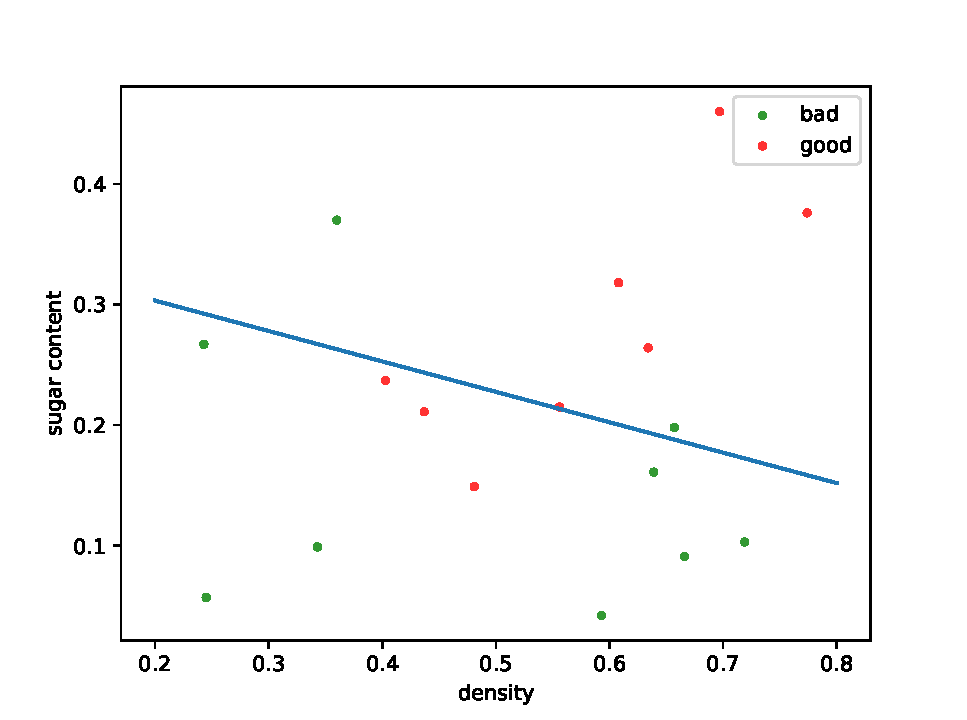
\includegraphics[scale=1,width=0.83\textwidth]{../image/3.3my.pdf}
		\caption{对数几率回归在西瓜数据集$3.0\alpha$上的结果。}
		\label{Logistic_RES}
	\end{figure}

	\begin{table}[htb]
		\centering
		\begin{tabular}{c|c|c}
			\hline
			\multirow{2}*{真实情况}& \multicolumn{2}{c}{预测结果}\\
			\cline{2-3}
			&正例&反例\\
			\hline
			正例&5&3\\
			\hline
			反例&2&7\\
			\hline
		\end{tabular}
		\caption{分类结果混淆矩阵}
		\label{Confusion_Mat}
	\end{table}

	网络上暂时找不到测试集,若将训练集作为测试集,则模型的分类混淆矩阵为表\ref{Confusion_Mat}。则查准率 $P=\frac{5}{5+2}=71.43\%$,查全率 $R=\frac{5}{8}=62.5\%$,总体准确率为 $\frac{12}{17}=70.59\%$。
	
	可以看出,由于数据集较少,模型的准确率并不是很高。如图\ref{迭代速度图},使用小规模的西瓜数据集$3.0\alpha$进行训练,$\bm{\beta}$收敛速度极快;若我们需要大规模的数据来训练模型以提高准确率,就需要消耗更长的时间得到最优解,但这样的牺牲在现如今的硬件条件下是可行的。
	
	\begin{figure}[htb]
		\centering
		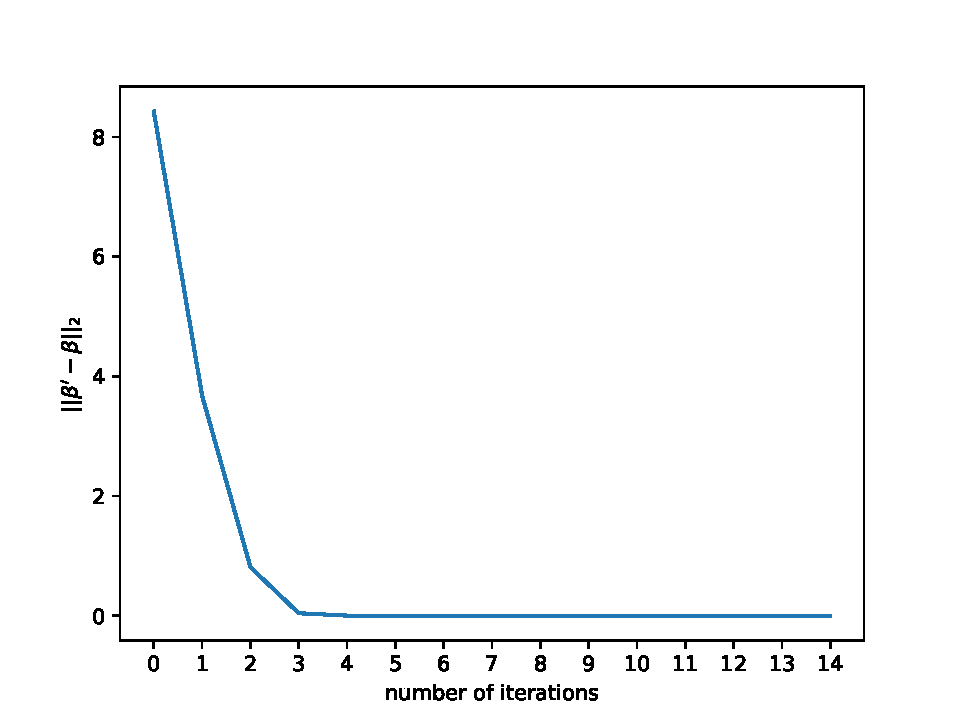
\includegraphics[scale=1,height=9cm]{../image/3.3迭代关系}
		\caption{迭代收敛速度}
		\label{迭代速度图}
	\end{figure}

	\subsection{学习收获}
	
	在对数几率回归这一节内容,我们使用了极大似然法来得到最优解;而在之前的线性回归一节中,我们使用最小二乘法来得到最优解。我认为这两种方法是得到最优解的不同角度,极大似然法要求趋近真实样本的概率极大,最小二乘法要求均方误差极小。针对回归问题,样本的真实值是不固定的,因此使用最小二乘法较为适合;针对分类问题,样本的真实标记为仅有的几个种类,使用极大似然法得到的模型能在预测未知样本时尽可能接近真实标记。
	
	与自己实现的对数几率回归相比,scikit-learn提供的函数支持不同的代价函数,可选择求解最优解的方法(梯度下降法、牛顿法等),设置迭代次数、误差范围等参数。
	\subsection{参考资料}   
	\begin{itemize}
		\item \href{https://scikit-learn.org.cn/view/378.html}{sklearn.linear\_model.LogisticRegression(scikit-learn中文社区)}
		\item\href{https://scikit-learn.org.cn/view/228.html}{Logistic回归三分类器(scikit-learn中文社区)}
		\item\href{https://scikit-learn.org.cn/view/4.html#1.1.11%20Logistic%E5%9B%9E%E5%BD%92}{线性模型(scikit-learn中文社区)}
		\item 《机器学习》3.3;周志华;清华大学出版社
		\item 《机器学习公式详解》3.27;谢文睿、秦州;人民邮电出版社
	\end{itemize}
	\section{习题3.4}
	\subsection{编程题目理解}
	题目要求,选择iris数据集,比较10折交叉验证和留一法所估计出的对率回归的错误率。
	
	10折交叉验证法和留一法只是划分数据集为训练集和测试集的两种方案,本身不涉及具体的数学原理,自己动手实现的意义不大;而且前面已经实现了对率回归算法,这里不再进行重复工作;我们不妨熟悉一下机器学习库scikit-learn,用其自带函数比较10折交叉验证和留一法。
	
	\subsection{交叉验证法阐述}
	“交叉验证法”先将数据集 $D$ 划分为 $k$ 个大小相似的互斥自己,即 $D=D_1\cup D_2\cup \cdots \cup D_k$,$D_i\cap D_j=\varnothing\ (i\neq j)$。每个子集 $D_i$ 都尽可能保持数据分布的一致性,即从 $D$ 中通过分层采样得到。然后,每次用 $k-1$ 个子集的并集作为训练集,余下的那个子集作为测试集;这样就可以得到 $k$ 组训练/测试集,从而可进行 $k$ 次训练和测试,最终返回的是这 $k$ 个测试结果的均值。
	
	当上述交叉验证的参数 $k=10$ 时,称为10折交叉验证。
	
	\begin{figure}[hbt]
		\centering
		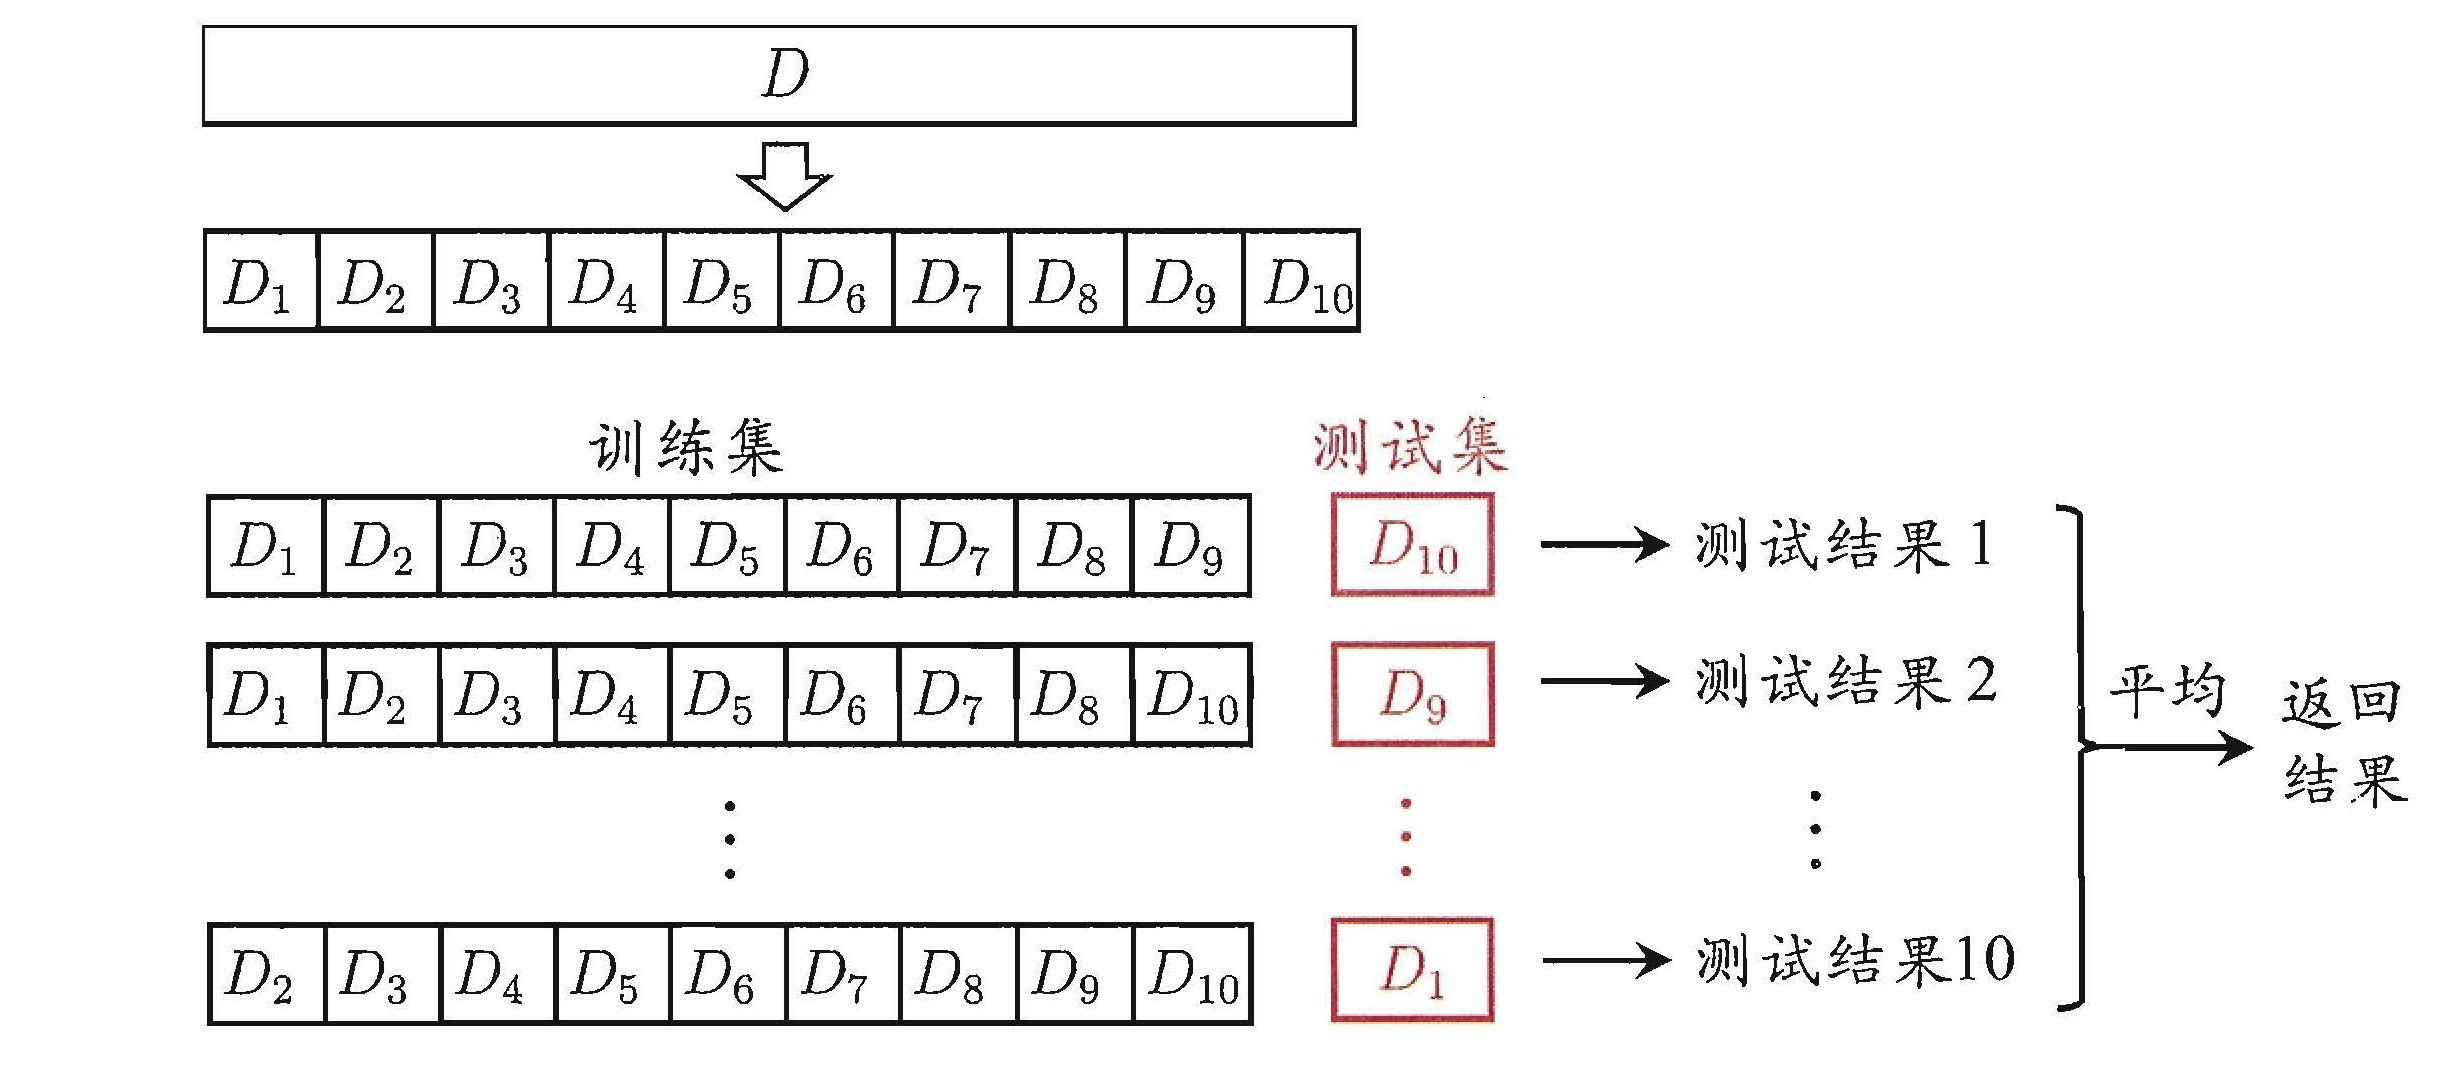
\includegraphics[scale=1,height=6cm]{../image/10折交叉验证.png}
		\caption{10折交叉验证}
	\end{figure}

	假定数据集 $D$ 中包含 $m$ 个样本,若令 $k=m$,则得到了交叉验证法的特例——留一法。显然,留一法不受随机样本划分方式的影响。
	
	\subsection{算法设计思路}
	
	iris数据集可从sklearn.datasets中获得。sklearn提供的iris降维示例如图\ref{iris数据集分类},可以发现iris共有三个分类,由于对数几率回归只能进行二分类任务,因此我们在代码中只取其中两个分类进行检验。
	
	\begin{figure}[htb]
		\centering
		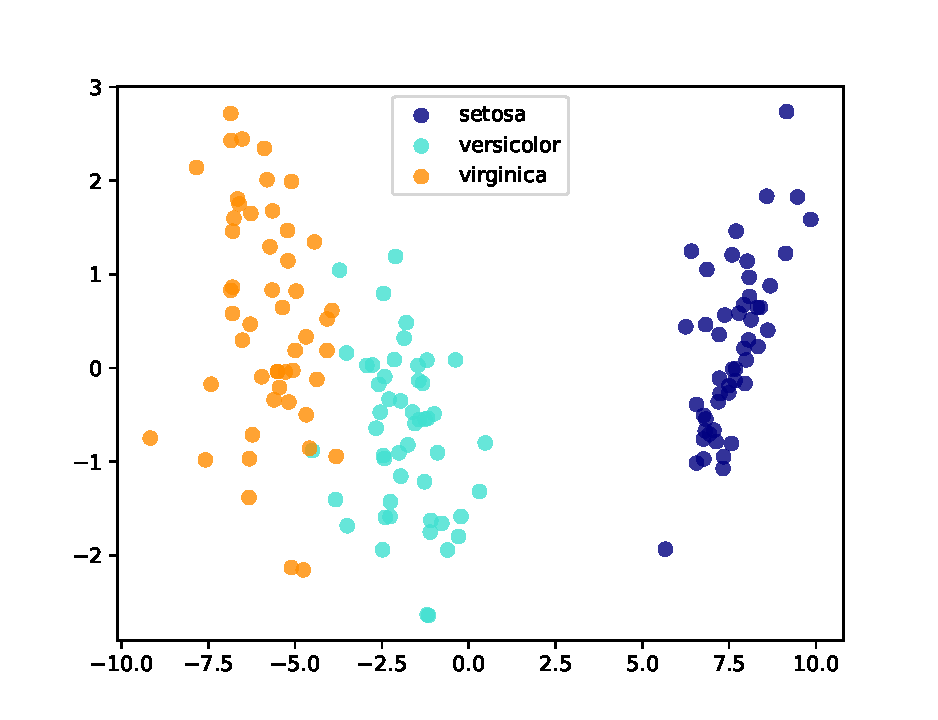
\includegraphics[scale=1,height=9.5cm]{../image/iris分类.pdf}
		\caption{iris数据集分类}
		\label{iris数据集分类}
	\end{figure}

	关于评估方法的对象都在sklearn.model\_selection软件包中,交叉验证法函数为cross\_val\_predict,留一法对象为LeaveOneOut。
	
	cross\_val\_predict为输入数据生成交叉验证的估计值。cross\_val\_predict接收对象estimator,作为拟合数据的模型,在这里就是对数几率回归对象LogisticRegression。在程序中,调用cross\_val\_predict需要指定模型estimator、数据集(iris的参数和真实值)、交叉验证参数 cv(10折交叉验证cv=10)。cross\_val\_predict返回预测结果数组,调用sklearn.metrics包中的accuracy\_score函数将预测值与真实值比较,可得到准确率。
	
	使用留一法检验,首先需要创建实例。调用LeaveOneOut.split函数可以将样分为训练集(99个)和测试集(1个),调用LogisticRegression.fit可以使用训练集训练对数几率回归模型,接着可用LogisticRegression.predict得到测试集的预测值。如此进行100次留一法检验,可得到最后的正确率。
	
	\subsection{核心代码分析}
	\subsubsection{取数据}
	iris数据集共有150个样本,每50个样本属于一个分类,共有 $C_3^2=3$ 种取分类的方法,检验时需要取100个只属于两个分类的样本。
	\lstinputlisting[style=Python]{../code/core/取数据3.4.txt}
	\subsubsection{定义模型}
	这里用对数几率回归检验错误率,因此定义模型LogisticRegression。
	\lstinputlisting[style=Python]{../code/core/定义模型3.4.txt}
	\subsubsection{10折交叉验证}
	调用cross\_val\_predict函数,得到预测值;调用accuracy\_score函数,得到正确率。
	\lstinputlisting[style=Python]{../code/core/10折交叉验证3.4.txt}
	\subsubsection{留一法}
	创建留一法实例leaveOneOut,调用其split函数,将数据集划分为测试集和训练集。共有100个样本,因此有100种划分方法,遍历每一个划分方案,统计预测正确的次数,可得到最终的正确率。
	\lstinputlisting[style=Python]{../code/core/留一法3.4.txt}
	\subsection{实验结果分析}
	
	下载\href{https://archive.ics.uci.edu/ml/machine-learning-databases/iris/iris.data}{iris数据集},可以看到共有setosa、versicolor、virginica三种鸢尾花,取不同的两种鸢尾花用于进行对数几率回归,得到结果如表\ref{3.4结果}。
	
	留一法使用的训练集与初始可以看到10折交叉验证法和留一法所估计出的对率回归的错误率在iris数据集上没有显示出明显的差别。因此,我尝试比较了多个 $k$ 折交叉验证的错误率,其中 $k\in\{2,3,5,10,15,30,50\}$,得到的结果如图\ref{错误率变化}。当 $k$ 逐渐增大,对率回归在iris数据集上的错误率逐渐减小,并最终达到留一法的错误率,并不再改变。从这一结果来看,对于机器学习算法得到的模型,其针对特定数据集的预测正确率似乎存在阈值,达到阈值后难以继续提高。
	依据\ref{错误率变化},我们可初步得到结论:留一法使用的训练集与与初始数据集相比只少了一个样本,这样就使得绝大多数情况下,留一法中被实际评估的模型与期望评估的用数据集 $D$ 训练出的模型很相似;因此,留一法的评估结果往往比较准确。
	
	\begin{table}[htb]
		\centering
		\begin{tabular}{|c|c|c|c|}
			\hline
			\multirow{2}*{评估方法}& \multicolumn{3}{c|}{错误率}\\
			\cline{2-4}
			&(setosa, versicolor)&(setosa, virginica)&(versicolor, virginica)\\
			\hline
			10折交叉验证&0.0000000000000000000\%&0.0000000000000000000\%&4.0000000000000035527\%\\
			\hline
			留一法&0.0000000000000000000\%&0.0000000000000000000\%&4.0000000000000035527\%\\
			\hline
		\end{tabular}
		\caption{分类结果混淆矩阵}
		\label{3.4结果}
	\end{table}

	\begin{figure}[htb]
		\centering
		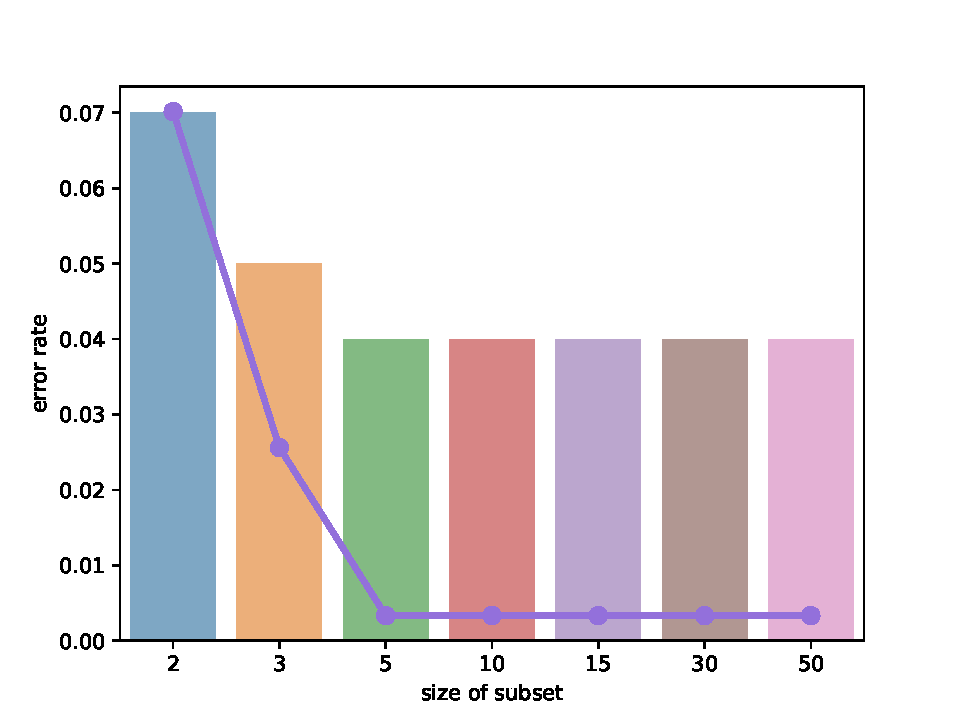
\includegraphics[scale=1,height=9.8cm]{../image/错误率变化.pdf}
		\caption{$k$折交叉验证错误率变化}
		\label{错误率变化}
	\end{figure}
	
	
	\subsection{学习收获}
	
	在本次实验中,我们使用对率回归对iris数据集分类,对率回归只能完成二分类任务,面对多类别的iris数据集显得有些捉襟见肘。
	
	通过查阅资料可知,将二分类的Logistic回归扩展,就是多分类的Softmax回归。Softmax函数能将 $n$ 维实向量“压缩”到另一个 $n$ 为实向量 $\sigma(z)$ 中,使得每个元素的范围都在 $[0,1]$ 之间,并且所有元素的和为 $1$。
	
	\begin{equation}
		\bm{\sigma}(\bm{z})_i=\frac{e^{z_i}}{\sum\limits_{k=1}^{n}e^{z_k}}
	\end{equation}

	假设有 $n$ 种分类,可以将分类的条件概率写成Softmax函数的形式
	
	\begin{equation}
		P(y_i=c)=\frac{e^{\bm{\beta}_c^\mathrm{T}\hat{\bm{x}}_i}}{\sum\limits_{k=1}^{n}e^{\bm{\beta}_k^\mathrm{T}\hat{\bm{x}}_i}}
	\end{equation}
	
	\subsection{参考资料}
	
	\begin{itemize}
		\item 《机器学习》2.2.2;周志华;清华大学出版社
		\item \href{https://blog.csdn.net/sai_simon/article/details/122470130}{多分类对数几率回归算法(CSDN sai\_simon)}
		\item \href{https://en.wikipedia.org/wiki/Multinomial_logistic_regression}{Multinomial logistic regression(Wikipedia)}
	\end{itemize}

	\section{习题3.5}
	\subsection{编程题目理解}
	
	题目要求编程实现线性判别分析,并给出西瓜数据集 $3.0\alpha$ 上的结果。
	
	在西瓜数据集 $3.0\alpha$ 中,西瓜包含“密度”和“含糖率”两个参数,因此可将西瓜看做横坐标为“密度”纵坐标为“含糖率”的坐标系中的点。使用LDA,就是要将这些代表西瓜的点投影到平面中的一条直线上,使得好瓜样例的投影点尽可能接近、坏瓜样例的投影点尽可能远离。
	
	\subsection{LDA原理阐述}
	\label{Section_LDA_Theory}
	
	LDA的思想非常朴素: 给定训练样例集,设法将样例投影到一条直线上,使得同类样例的投影点尽可能接近、异类样例的投影点尽可能远离;在对新样本进行分类时,将其投影到同样的这条直线上,再根据投影点的位置来确定新样本的类别。
	
	\begin{figure}[htb]
		\centering
		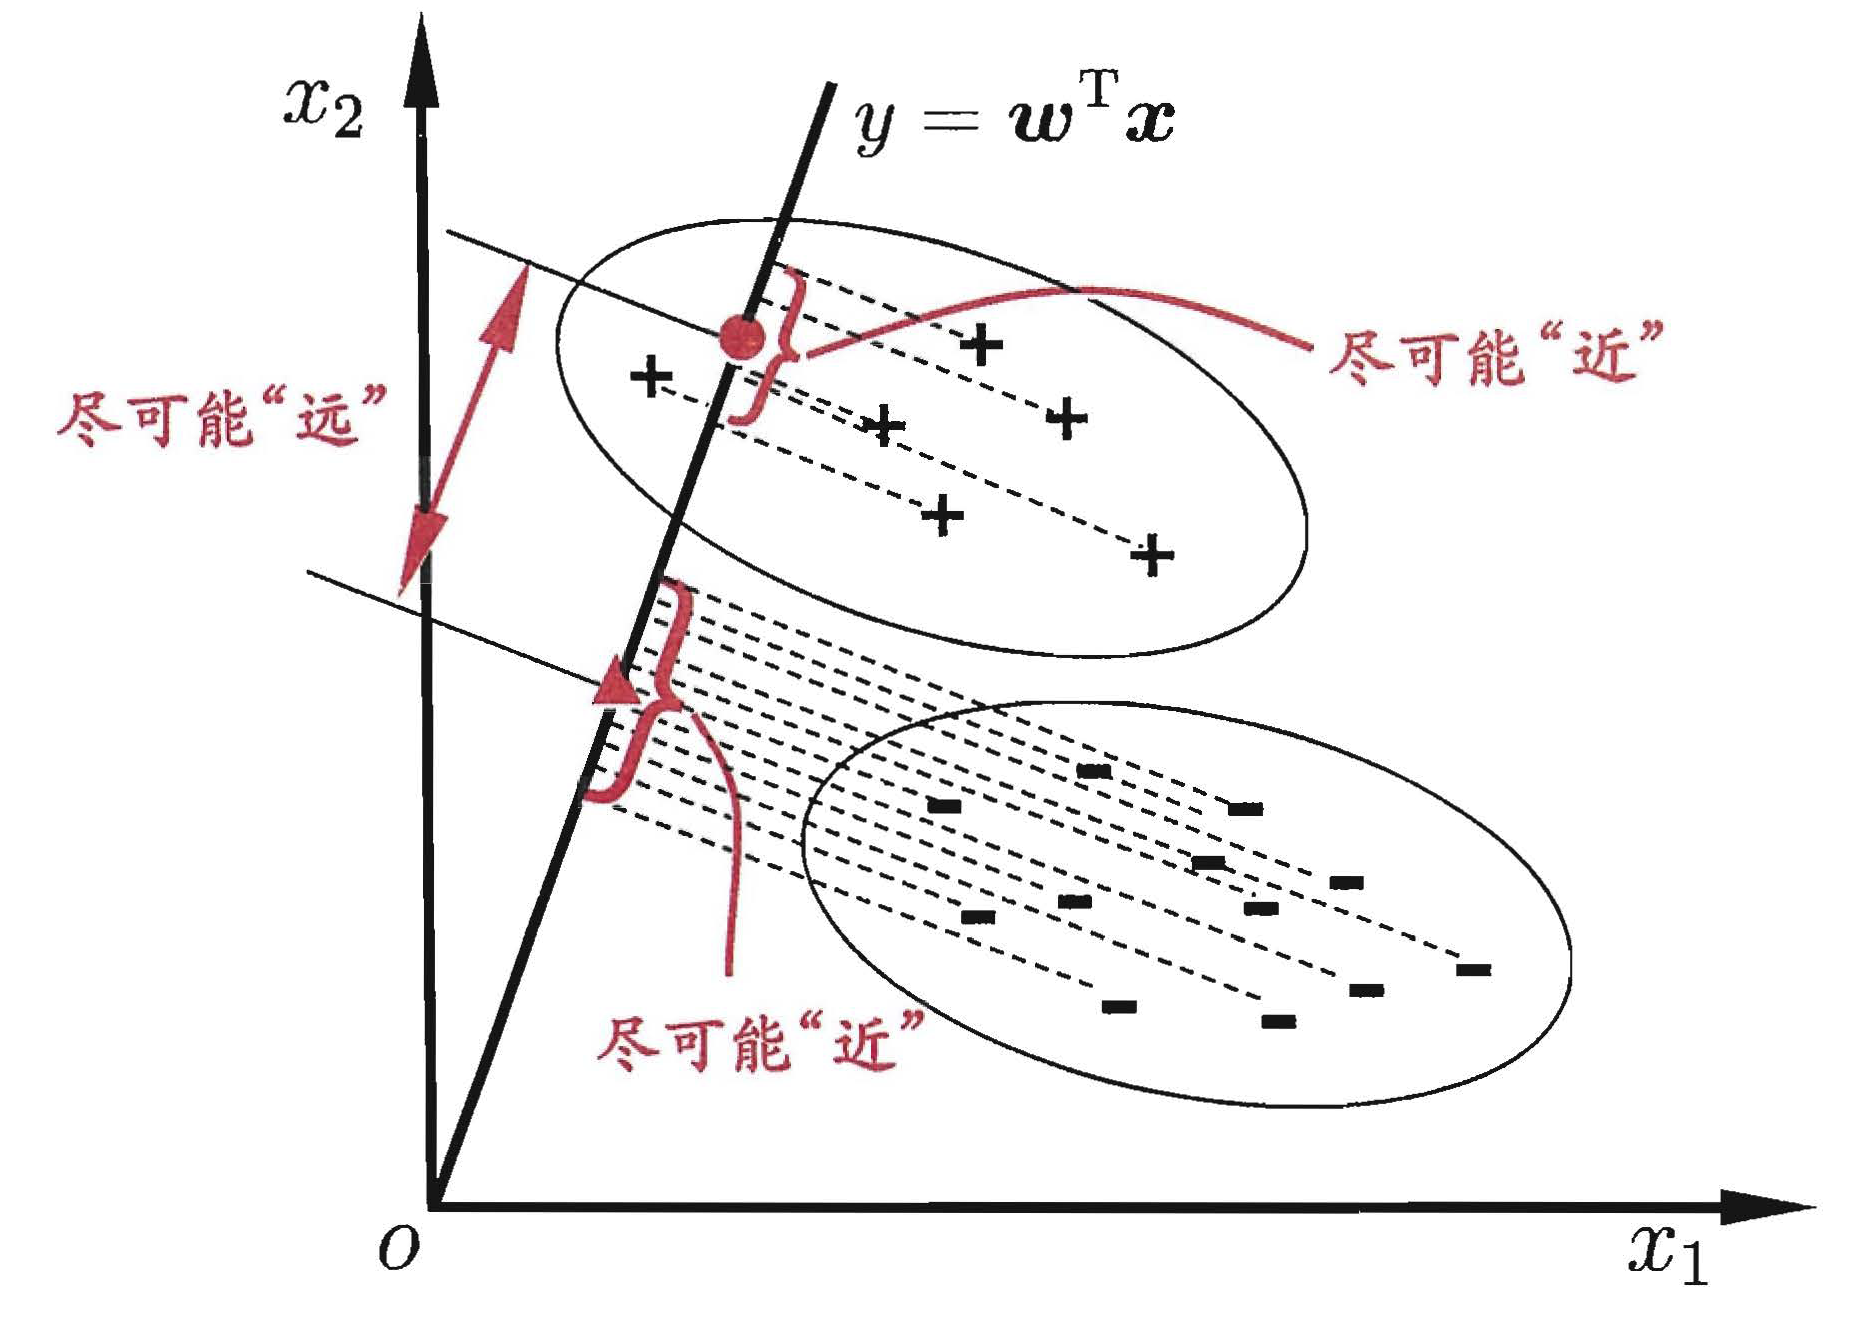
\includegraphics[scale=1,height=6cm]{../image/LDA-example.png}
		\caption{LDA二维示意图}
		\label{LDA-example}
	\end{figure}

	对于二分类问题,给定数据集 $D=\{(\bm{x}_i,y_i)\}_{i=1}^{m}$,$y_i\in\{0,1\}$,令 $X_i$、$\bm{\mu}_i$、$\bm{\Sigma}_i$ 分别表示第 $i\in\{0,1\}$ 类示例的集合、均值向量、协方差矩阵。若将数据投影到过原点的直线 $\bm{w}$ 上,则两类样本的中心在直线上的投影分别为 $\bm{w}^\mathrm{T}\bm{\mu}_0$ 和 $\bm{w}^\mathrm{T}\bm{\mu}_1$;若将所有样本点都投影到直线上,则两类样本的协方差分别为 $\bm{w}^\mathrm{T}\bm{\Sigma}_0\bm{w}$ 和 $\bm{w}^\mathrm{T}\bm{\Sigma}_1\bm{w}$。由于直线是一维空间,因此 $\bm{w}^\mathrm{T}\bm{\mu}_0$、$\bm{w}^\mathrm{T}\bm{\mu}_1$、$\bm{w}^\mathrm{T}\bm{\Sigma}_0\bm{w}$、$\bm{w}^\mathrm{T}\bm{\Sigma}_1\bm{w}$ 均为实数。
	
	
	欲使同类样例的投影点尽可能接近,可以让同类样例投影点的协方差尽可能小,即 $\bm{w}^\mathrm{T}\bm{\Sigma}_0\bm{w}+\bm{w}^\mathrm{T}\bm{\Sigma}_1\bm{w}$ 尽可能小;而欲使异类样例的投影点尽可能远离,可以让类中心之间的距离尽可能大,即 $||\bm{w}^\mathrm{T}\bm{\mu}_0-\bm{w}^\mathrm{T}\bm{\mu}_1||_2^2$ 尽可能大。同时考虑二者,则可得到欲最大化的目标
	
	\begin{equation}
		\begin{aligned}
			J&=\frac{||\bm{w}^\mathrm{T}\bm{\mu}_0-\bm{w}^\mathrm{T}\bm{\mu}_1||_2^2}{\bm{w}^\mathrm{T}\bm{\Sigma}_0\bm{w}+\bm{w}^\mathrm{T}\bm{\Sigma}_1\bm{w}}\\
			&=\frac{\bm{w}^\mathrm{T}(\bm{\mu}_0-\bm{\mu}_1)[\bm{w}^\mathrm{T}(\bm{\mu}_0-\bm{\mu}_1)]^\mathrm{T}}{\bm{w}^\mathrm{T}\bm{\Sigma}_0\bm{w}+\bm{w}^\mathrm{T}\bm{\Sigma}_1\bm{w}}\\
			&=\frac{\bm{w}^\mathrm{T}(\bm{\mu}_0-\bm{\mu}_1)(\bm{\mu}_0-\bm{\mu}_1)^\mathrm{T}\bm{w}}{\bm{w}^\mathrm{T}\bm{\Sigma}_0\bm{w}+\bm{w}^\mathrm{T}\bm{\Sigma}_1\bm{w}}\label{Initial_J}
		\end{aligned}
	\end{equation}
	
	定义“类内散度矩阵”
	
	\begin{equation}
		\label{EQ_Sw}
		\begin{aligned}
			\mathbf{S}_w&=\bm{\Sigma}_0+\bm{\Sigma}_1\\
			&=\sum_{\bm{x}\in X_0}(\bm{x}-\bm{\mu}_0)(\bm{x}-\bm{\mu}_0)^\mathrm{T}+\sum_{\bm{x}\in X_1}(\bm{x}-\bm{\mu}_1)(\bm{x}-\bm{\mu}_1)^\mathrm{T}
		\end{aligned}
	\end{equation}
	
	定义“类间散度矩阵”
	
	\begin{equation}
		\mathbf{S}_b=(\bm{\mu}_0-\bm{\mu_1})(\bm{\mu}_0-\bm{\mu_1})^\mathrm{T}
	\end{equation}
	
	则式\eqref{Initial_J}可重写为
	
	\begin{equation}
		J=\frac{\bm{w}^\mathrm{T}\mathbf{S}_b\bm{w}}{\bm{w}^\mathrm{T}\mathbf{S}_w\bm{w}}
		\label{Final_J}
	\end{equation}

	注意到式\eqref{Final_J}的分子和分母都是关于 $\bm{w}$ 的二次项,因此式\eqref{Final_J}的解与 $\bm{w}$ 的长度无关,只与其方向有关,这一点从图\ref{LDA-example}中可以直观看出。不失一般性,令 $\bm{w}^\mathrm{T}\mathbf{S}_w\bm{w}=1$,则式\eqref{Final_J}等价于
	
	\begin{equation}
		\begin{aligned}
			\min_{\bm{w}}\quad &-\bm{w}^\mathrm{T}\mathbf{S}_b\bm{w}\\
			\text{s.t.}\quad &\bm{w}^\mathrm{T}\mathbf{S}_w\bm{w}=1
		\end{aligned}
		\label{Constraint_J}
	\end{equation}

	根据式\eqref{Constraint_J},可构造Lagrange函数
	
	\begin{equation}
		L(\bm{w},\lambda)=-\bm{w}^\mathrm{T}\mathbf{S}_b\bm{w}+\lambda(\bm{w}^\mathrm{T}\mathbf{S}_w\bm{w}-1)
	\end{equation}

	已知
	
	\begin{equation}
		\begin{aligned}
			\frac{\partial L(\bm{w},\lambda)}{\partial\bm{w}}&=\frac{\partial}{\partial\bm{w}}[-\bm{w}^\mathrm{T}\mathbf{S}_b\bm{w}+\lambda(\bm{w}^\mathrm{T}\mathbf{S}_w\bm{w}-1)]\\
			&=-\frac{\partial(\bm{w}^\mathrm{T}\mathbf{S}_b\bm{w})}{\partial\bm{w}}+\frac{\partial(\lambda\bm{w}^\mathrm{T}\mathbf{S}_w\bm{w})}{\partial\bm{w}}-\frac{\partial\lambda}{\partial\bm{w}}\\
			&=-(\mathbf{S}_b+\mathbf{S}_b^\mathrm{T})\bm{w}+\lambda(\mathbf{S}_w+\mathbf{S}_w^\mathrm{T})\bm{w}\\
			&=-2\mathbf{S}_b\bm{w}+2\lambda\mathbf{S}_w\bm{w}
		\end{aligned}
	\end{equation}

	令 $\frac{\partial L(\bm{w},\lambda)}{\partial\bm{w}}=0$,则有 $\mathbf{S}_b\bm{w}=\lambda\mathbf{S}_w\bm{w}$,即 $(\bm{\mu}_0-\bm{\mu_1})(\bm{\mu}_0-\bm{\mu_1})^\mathrm{T}\bm{w}=\lambda\mathbf{S}_w\bm{w}$。由于 $(\bm{\mu}_0-\bm{\mu_1})^\mathrm{T}\bm{w}$ 为实数且矩阵乘法满足结合律,因此 $\mathbf{S}_b\bm{w}$ 为 $(\bm{\mu}_0-\bm{\mu}_1)$ 方向的向量;我们并不关心 $\lambda$ 的数值,并且 $\bm{w}$ 的长度也不影响结果,所以不妨令 $\mathbf{S}_b\bm{w}=\lambda(\bm{\mu}_0-\bm{\mu}_1)$,得到最终结果
	
	\begin{equation}
		\bm{w}=\mathbf{S}_w^{-1}(\bm{\mu}_0-\bm{\mu}_1)
	\end{equation}

	\subsection{LDA算法设计思路}
	\label{LDA_Idea}
	西瓜包含“密度”和“含糖率”两个参数,因此可将西瓜看做横坐标为“密度”纵坐标为“含糖率”的坐标系中的向量 $\bm{x}_i=\begin{pmatrix}x_{i1}\\x_{i2}\end{pmatrix}$。正例和反例分别组成矩阵 $X_1=\begin{pmatrix}\bm{x}_{1}^\mathrm{T}\\\bm{x}_{2}^\mathrm{T}\\\vdots\\\bm{x}_{8}^\mathrm{T}\end{pmatrix}$ 和 $X_0=\begin{pmatrix}\bm{x}_{9}^\mathrm{T}\\\bm{x}_{10}^\mathrm{T}\\\vdots\\\bm{x}_{17}^\mathrm{T}\end{pmatrix}$,我们可以使用NumPy的ndarray类型表示这一矩阵结构。接着就可以调用“np.mean(X, axis=0).reshape((2, 1))”得到均值向量 $\bm{\mu}_i$,注意这里的均值向量为二维列向量。然后需要计算协方差矩阵,已知 $\Sigma_i=\sum\limits_{\bm{x}\in X_i}(\bm{x}-\bm{\mu}_i)(\bm{x}-\bm{\mu}_i)^\mathrm{T}$,因此需要将代码中的反例和正例矩阵转置后与均值向量相减,在代码中表示为“Sigma = (X.T - mu) @ (X.T - mu).T”。类内散度矩阵就是两个协方差矩阵的简单相加,可写成“Sw = Sigma0 + Sigma1”。最后调用NumPy求解矩阵逆的函数,可计算得到直线向量 $\bm{w}$,“w = np.linalg.inv(Sw) @ (mu0 - mu1)”。计算流程如图\ref{LDA_Cal}。
	
	\begin{figure}[htb]
		\centering
		\scriptsize  
		%定义语句块的颜色,形状和边
		\tikzstyle{format}=[rectangle,draw,thin,fill=white]
		\begin{tikzpicture}
			\node[format](define){\large 定义数据集};
			\node[format,right of=define,node distance=50mm](calMu){\large 计算均值向量 $\bm{\mu}_i=\frac{1}{\sum\limits_{\bm{x}}[\bm{x}\in X_i]}\sum\limits_{\bm{x}\in X_i}\bm{x}$};
			\node[format,right of=calMu,node distance=74mm](calSigma){\large 计算协方差矩阵 $\Sigma_i={X_i^\mathrm{T}}-(\bm{\mu}_i;\bm{\mu}_i;\cdots)$};
			\node[format,below of=calSigma,node distance=12mm](Sw){\large 计算类内散度矩阵 $\mathbf{S}_w=\Sigma_0+\Sigma_1$};
			\node[format,left of=Sw,node distance=70mm](w){\large 得到直线 $\bm{w}=\mathrm{S}_w(\bm{mu}_0-\bm{\mu}_1)$};
			\draw[->](define)--(calMu);
			\draw[->](calMu)--(calSigma);
			\draw[->](calSigma)--(Sw);
			\draw[->](Sw)--(w);
		\end{tikzpicture}
		\caption{LDA计算流程}
		\label{LDA_Cal}
	\end{figure}  
	
	在得到直线 $\bm{w}$ 后,我们可以借用matplotlib库画出投影的图形。首先,调用scatter函数可画出原始点的位置,调用plot函数可画出直线 $\bm{w}$。我们主要考虑如何计算得到投影后的点。已知直线向量为 $\bm{w}$,原始点表示的向量为 $\bm{x}$,那么两向量点积 $\bm{w}\cdot\bm{x}=||\bm{w}||_2||x||_2\cos<\bm{w},\bm{x}>$,于是有投影 $d=||\bm{x}||_2\cos<\bm{w},\bm{x}>=\frac{\bm{w}\cdot\bm{x}}{||\bm{w}||_2}$。设 $\bm{w}=\begin{pmatrix}w_1\\w_2\end{pmatrix}$,则直线同 $x$ 轴夹角 $\theta=\arctan\frac{w_2}{w_1}$,投影点坐标为 $(d\cos\theta,d\sin\theta)$。在代码中,可调用NumPy的数学函数得到投影点坐标。
	
	\subsection{核心代码详解}
	\subsubsection{数据集格式}
	好瓜和坏瓜都用NumPy的ndarry格式存储,构成矩阵 $X=\begin{pmatrix}\bm{x}^\mathrm{T}\\\vdots\end{pmatrix}$,数组y表示瓜的好坏。\\
	\lstinputlisting[style=Python]{../code/core/data3.5.txt}
	\subsubsection{LDA(实现)}
	\label{LDA_MY}
	均值向量 $\bm{\mu}_i=\sum\limits_{\bm{x}\in X_i}\bm{x}$,因此需要对矩阵 $X_i$ 中的各个行向量求平均,并转为符合\ref{Section_LDA_Theory}公式推导的列向量。接着可按式\eqref{EQ_Sw}计算协方差矩阵得到类内散度矩阵 $\mathbf{S}_w$。最后调用NumPy库求逆矩阵函数numpy.linalg.inv得到直线方向向量。计算得到的直线方向向量需要做一定修正,使其方向朝向y正半轴,方便接下来计算投影点坐标。
	\lstinputlisting[style=Python]{../code/core/cal3.5.txt}
	\subsubsection{绘制图像}
	根据\ref{LDA_Idea}处的推导,计算投影点的函数如下。函数首先计算得到投影点与原点之间的距离,再根据向量与x正半轴的夹角,得到投影点的坐标。
	\lstinputlisting[style=Python]{../code/core/projection.txt}
	
	首先绘制原始点,根据原始点得到投影点,最后将原始点和投影点连线,得到垂直于投影直线的线段。
	\lstinputlisting[style=Python]{../code/core/draw3.5.txt}
	\subsubsection{调用scikit-learn}
	scikit-learn库提供了类LinearDiscriminantAnalysis,我们可以使用该类实施LDA降维。对于西瓜数据集 $3.0\alpha$,其属性coef\_即为直线向量 $\bm{w}$。
	\lstinputlisting[style=Python]{../code/core/sk3.5.txt}
	
	\subsection{实验结果分析}
	
	运行代码,解得$\bm{w}=\begin{pmatrix}0.14650982\\0.73871557\end{pmatrix}$,即直线斜率为 $5.04208922$,在西瓜数据集 $3.0\alpha$ 上得到的结果如图\ref{LDA_RES}。
	
	\begin{figure}[htb]
		\centering
		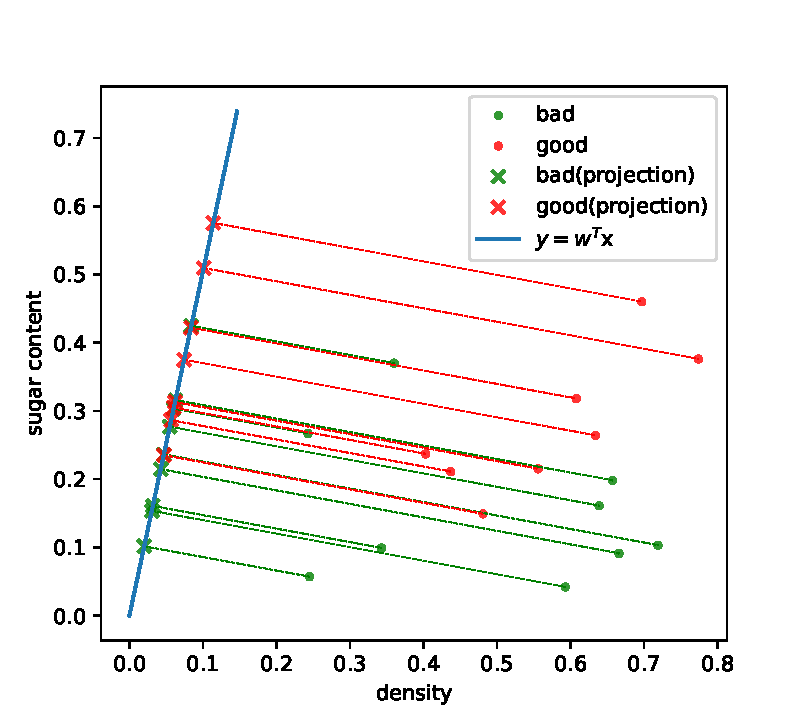
\includegraphics[scale=1,height=10.2cm]{../image/3.5my.pdf}
		\caption{LDA在西瓜数据集 $3.0\alpha$ 上的结果。}
		\label{LDA_RES}
	\end{figure}
	
	可以看到,在西瓜数据集 $3.0\alpha$ 上,LDA的分类效果并不显著,有一些坏瓜(绿点)和好瓜(红点)在投影后距离相差较小,这可能是训练集规模较小造成的。此外,LDA降维的意义应当大于分类。
	
	\subsection{学习收获}
	
	在章节\ref{Section_LDA_Theory},我们直接取均值向量投影为 $\bm{w}^\mathrm{T}\bm{\mu}_i$,这曾是我的一大疑点。已知直线方向向量 $\bm{w}$,那么向量 $\bm{x}$ 在直线上的投影为 $\frac{\bm{w}\cdot\bm{x}}{||\bm{w}||_2}$,即 $\frac{1}{||\bm{w}||_2}\bm{w}^\mathrm{T}\bm{x}$;仅在 $\bm{w}$ 为单位向量时,投影为 $\bm{w}^\mathrm{T}\bm{x}$。因此接下来的所有推导时理应都会包含 $\frac{1}{||\bm{w}||_2^k}$ 这一系数,其中 $k\in \mathbb{N}$。因为投影与 $||\bm{w}||_2$ 并无关系,因此我们不妨直接将这项系数丢弃,并灵活利用这一性质在推导中简化计算。
	
	在本次实验中,LDA将二维的西瓜数据投射到了一维的直线上;对此加以扩展,将 $\bm{W}$ 视为一个投影矩阵,则多分类LDA就可以将样本投影到$d'$空间,其中 $d'$ 一般远小于原有的属性 $d$。于是们可通过这个投影来减小样本点的尾数,因此LDA是一种使用了类别信息的监督降维技术。
	
	与自己实现的LDA相比,scikit-learn提供的函数能实施高维向量向低维向量的投影,同时支持奇异值分解、最小二乘解、特征值分解三种求解方式,且可以设置收缩参数、先验概率、奇异值阈值等参数。
	
	\subsection{参考资料}
	\begin{itemize}
		\item \href{https://scikit-learn.org.cn/view/618.html}{sklearn.discriminant\_analysis.LinearDiscriminantAnalysis(scikit-learn中文社区)}
		\item\href{http://scikit-learn.org.cn/view/152.html}{Iris数据集LDA和PCA二维投影的比较(scikit-learn中文社区)}
		\item 《机器学习》3.4;周志华;清华大学出版社
		\item 《机器学习公式详解》3.37;谢文睿、秦州;人民邮电出版社
	\end{itemize}
\end{document}
